
\begin{frame}
  \frametitle{Nuclear Forensics: Why?}
  \begin{figure}
    \centering
    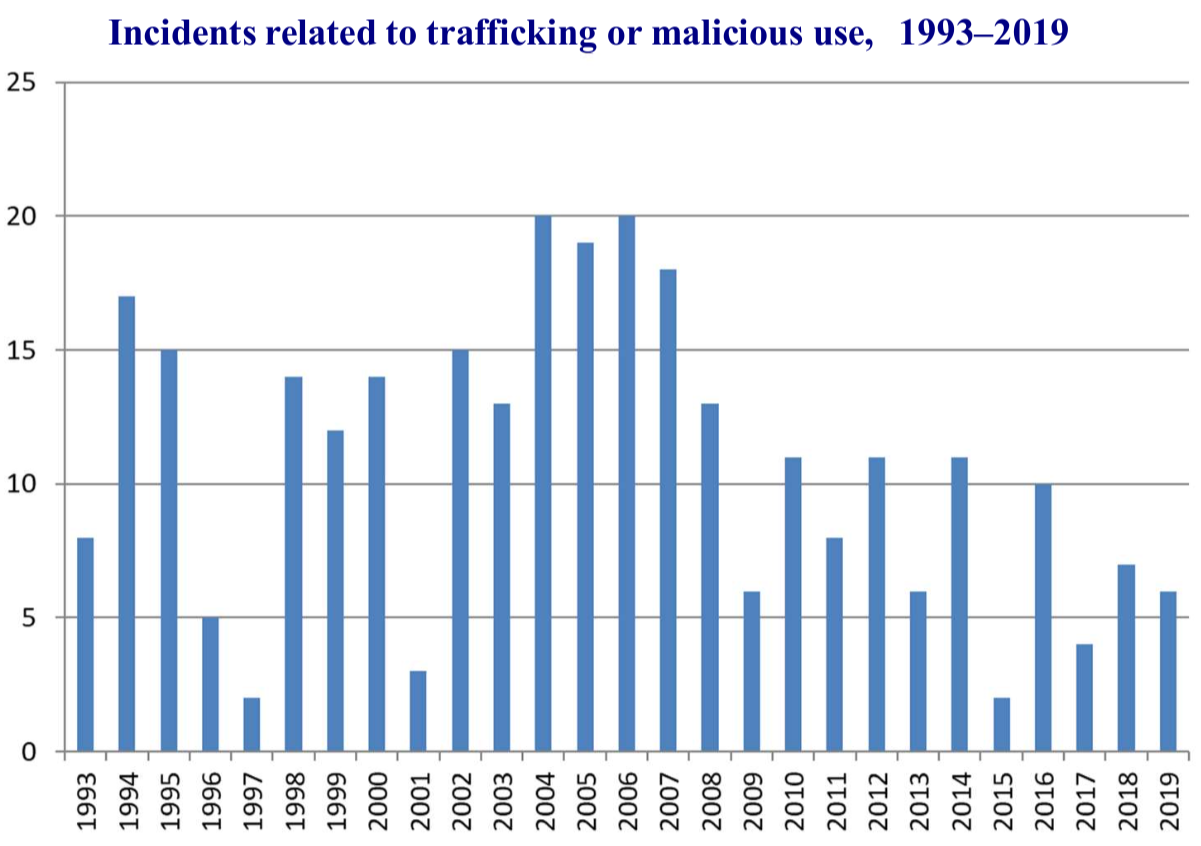
\includegraphics[width=0.78\textwidth]{./figures/nucleartrafficking.png}
  \end{figure}
  Incidents of highest concern: Highly enriched uranium (12), plutonium (2), 
  plutonium-beryllium neutron sources (5) \cite{itdb}
\end{frame}

\begin{frame}
  \frametitle{Nuclear Forensics Definition}
  \vspace{-8pt}
  \begin{figure}
    \centering
    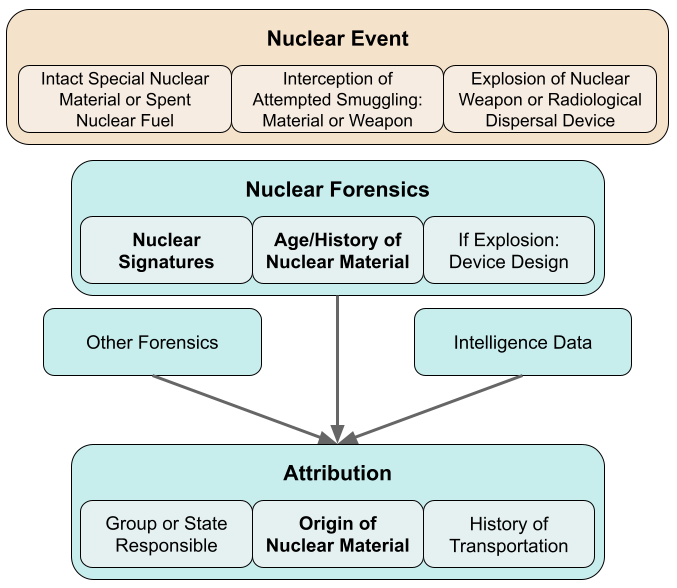
\includegraphics[height=0.9\textheight]{./figures/nf_define.png}
  \end{figure}
\end{frame}

\begin{frame}
  \frametitle{Nuclear Forensics Timelines}
  \begin{adjustwidth}{-10pt}{-15pt}
  \begin{figure}
    \centering
    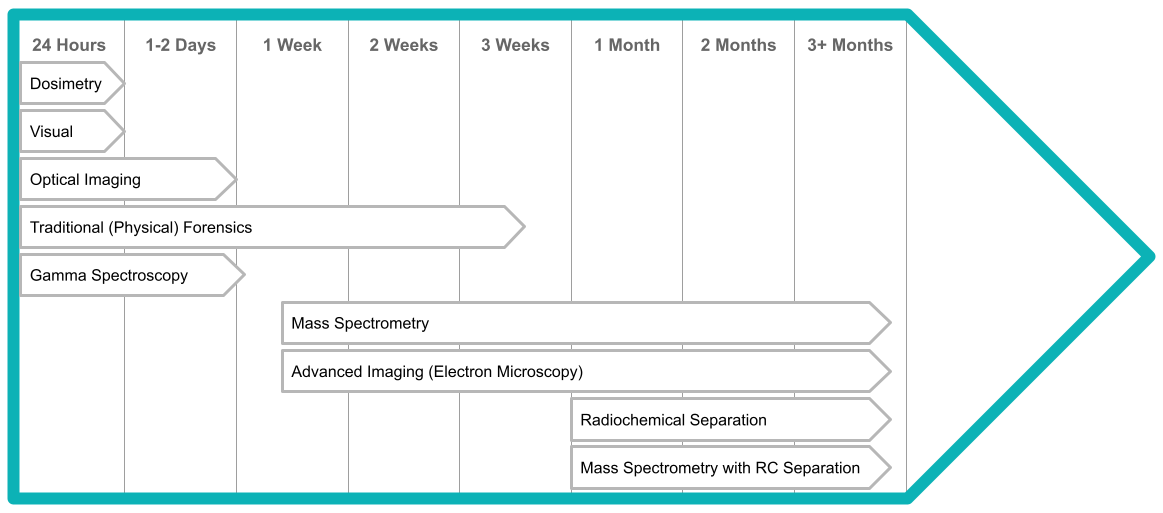
\includegraphics[width=1.1\textwidth]{./figures/nf_timeline.png}
    \\ \raggedright \scriptsize Author recreated from 
    \href{https://fas.org/pir-pubs/the-false-hope-of-nuclear-forensics-assessing-the-timeliness-of-forensics-intelligence/}{\color{blue}online
    article} by Eric Feigl-Ding.
  \end{figure}
  \end{adjustwidth}
\end{frame}

\begin{frame}
  \frametitle{Main Goal}

  Is it possible to \textbf{speed up} a nuclear forensics
  \textbf{investigation} of spent nuclear fuel with \textbf{field-deployable
  detection}?

\end{frame}

\begin{frame}
  \frametitle{Statistical Methods}
  \begin{itemize}
    \item Minimal domain knowledge to implement
    \item Enables the use of large numbers of simulations
    \item Opens up the possibility of using measurement techniques that are fast \& require little training
  \end{itemize}
\end{frame}

